% -*-TeX root = TM.tex
%%%%%%%%%%%%%%%%%%%%%%%%%%%%%%%%%%%%%%%%%
% The Legrand Orange Book
% LaTeX Template
% Version 2.1.1 (14/2/16)
%
% This template has been downloaded from:
% http://www.LaTeXTemplates.com
%
% Original author:
% Mathias Legrand (legrand.mathias@gmail.com) with modifications by:
% Vel (vel@latextemplates.com)% 
%
% License:
% CC BY-NC-SA 3.0 (http://creativecommons.org/licenses/by-nc-sa/3.0/)
%
% Important note:
% Chapter heading images should have a 2:1 width:height ratio,
% e.g. 920px width and 460px height.
%
%%%%%%%%%%%%%%%%%%%%%%%%%%%%%%%%%%%%%%%%%

% LATEXING SHORTCUTS
% cmd + l : fill a blank (for references…)
% cmd + maj + b : build 
% cmd + ctrl + b : custom build option
% cmd + l, cmd + b : build option
% cmd + l, cmd + o : open the pdf
% cmd + l, cmd + d : online lookup 
% § : insert symbol
% cmd + l, cmd + n : create new environement
% cmd + l, cmd + s : show snippets
% cmd + l, cmd + w, b | e | u : make the selectioned text bold | italic | undeline
% tab : escape character
% @ : snippets for bibtex
% cmd + l, cmd + p : show all the commands
% cmd + r : jump in the text (following structure)
% cmd + number : jump to specified tab

%----------------------------------------------------------------------------------------
%	PACKAGES AND OTHER DOCUMENT CONFIGURATIONS
%----------------------------------------------------------------------------------------

\documentclass[12pt,fleqn,oneside,openany]{book} % Paramètres

%----------------------------------------------------------------------------------------
%	VARIOUS REQUIRED PACKAGES
%----------------------------------------------------------------------------------------

\usepackage[top=3cm,bottom=3cm,left=3.2cm,right=3.2cm,headsep=10pt,a4paper]{geometry} % Page margins

\usepackage{xcolor} % Required for specifying colors by name
\definecolor{ocre}{RGB}{211, 84, 0} % couleur du doc

\usepackage{titlesec} % Allows customization of titles

\usepackage{graphicx} % Required for including pictures
\graphicspath{{img/}} % Specifies the directory where pictures are stored

\usepackage{lipsum} % Inserts dummy text

\usepackage{tikz} % Required for drawing custom shapes

\usepackage[francais]{babel} % Tout ce qu'il faut pour supporter un texte écrit en français

\usepackage{enumitem} % Customize lists
\setlist{nolistsep} % Reduce spacing between bullet points and numbered lists

\usepackage{booktabs} % Required for nicer horizontal rules in tables

\usepackage{eso-pic} % Required for specifying an image background in the title page

\usepackage{pdfpages} % pour les annexes

%----------------------------------------------------------------------------------------
%	POLICES
%----------------------------------------------------------------------------------------

% Font Settings
\usepackage{avant} % Use the Avantgarde font for headings
%\usepackage{times} % Use the Times font for headings
\usepackage{mathptmx} % Use the Adobe Times Roman as the default text font together with math symbols from the Sym­bol, Chancery and Com­puter Modern fonts

\usepackage{microtype} % Slightly tweak font spacing for aesthetics
\usepackage[utf8]{inputenc} % Required for including letters with accents
\usepackage[T1]{fontenc} % Use 8-bit encoding that has 256 glyphs

%----------------------------------------------------------------------------------------
%	MAIN TABLE OF CONTENTS
%----------------------------------------------------------------------------------------

\usepackage{titletoc} % Required for manipulating the table of contents

\contentsmargin{0cm} % Removes the default margin
% Chapter text styling
\titlecontents{chapter}[1.25cm] % Indentation
{\addvspace{15pt}\large\sffamily\bfseries} % Spacing and font options for chapters
{\color{ocre!60}\contentslabel[\Large\thecontentslabel]{1.25cm}\color{ocre}} % Chapter number
{}  
{\color{ocre!60}\normalsize\sffamily\bfseries\;\titlerule*[.5pc]{.}\;\thecontentspage} % Page number
% Section text styling
\titlecontents{section}[1.25cm] % Indentation
{\addvspace{5pt}\sffamily\bfseries} % Spacing and font options for sections
{\contentslabel[\thecontentslabel]{1.25cm}} % Section number
{}
{\sffamily\hfill\color{black}\thecontentspage} % Page number
[]
% Subsection text styling
\titlecontents{subsection}[1.25cm] % Indentation
{\addvspace{1pt}\sffamily\small} % Spacing and font options for subsections
{\contentslabel[\thecontentslabel]{1.25cm}} % Subsection number
{}
{\sffamily\;\titlerule*[.5pc]{.}\;\thecontentspage} % Page number
[] 

%----------------------------------------------------------------------------------------
%	MINI TABLE OF CONTENTS IN CHAPTER HEADS
%----------------------------------------------------------------------------------------

% Section text styling
\titlecontents{lsection}[0em] % Indendating
{\footnotesize\sffamily} % Font settings
{}
{}
{}

% Subsection text styling
\titlecontents{lsubsection}[.5em] % Indentation
{\normalfont\footnotesize\sffamily} % Font settings
{}
{}
{}
 
%----------------------------------------------------------------------------------------
%	PAGE HEADERS
%----------------------------------------------------------------------------------------

\usepackage{fancyhdr} % Required for header and footer configuration

\pagestyle{fancy}
\renewcommand{\chaptermark}[1]{\markboth{\sffamily\normalsize\bfseries\chaptername\ \thechapter.\ #1}{}} % Chapter text font settings
\renewcommand{\sectionmark}[1]{\markright{\sffamily\normalsize\thesection\hspace{5pt}#1}{}} % Section text font settings
\fancyhf{} \fancyhead[RO]{\sffamily\normalsize\thepage} % Font setting for the page number in the header
\fancyhead[L]{\leftmark} % Print the current chapter name on the left side of  page

\renewcommand{\headrulewidth}{0.5pt} % Width of the rule under the header
\addtolength{\headheight}{2.5pt} % Increase the spacing around the header slightly
\renewcommand{\footrulewidth}{0pt} % Removes the rule in the footer
\fancypagestyle{plain}{\fancyhead{}\renewcommand{\headrulewidth}{0pt}} % Style for when a plain pagestyle is specified

% Removes the header from odd empty pages at the end of chapters
\makeatletter
\renewcommand{\cleardoublepage}{
\clearpage\ifodd\c@page\else
\hbox{}
\vspace*{\fill}
\thispagestyle{empty}
\newpage
\fi}

%----------------------------------------------------------------------------------------
%	THEOREM STYLES
%----------------------------------------------------------------------------------------

\usepackage{amsmath,amsfonts,amssymb,amsthm} % For math equations, theorems, symbols, etc

\newcommand{\intoo}[2]{\mathopen{]}#1\,;#2\mathclose{[}}
\newcommand{\ud}{\mathop{\mathrm{{}d}}\mathopen{}}
\newcommand{\intff}[2]{\mathopen{[}#1\,;#2\mathclose{]}}
\newtheorem{notation}{Notation}[chapter]

%%%%%%%%%%%%%%%%%%%%%%%%%%%%%%%%%%%%%%%%%%%%%%%%%%%%%%%%%%%%%%%%%%%%%%%%%%%
%%%%%%%%%%%%%%%%%%%% dedicated to boxed/framed environements %%%%%%%%%%%%%%
%%%%%%%%%%%%%%%%%%%%%%%%%%%%%%%%%%%%%%%%%%%%%%%%%%%%%%%%%%%%%%%%%%%%%%%%%%%
\newtheoremstyle{ocrenumbox}% % Theorem style name
{0pt}% Space above
{0pt}% Space below
{\normalfont}% % Body font
{}% Indent amount
{\small\bf\sffamily\color{ocre}}% % Theorem head font
{\;}% Punctuation after theorem head
{0.25em}% Space after theorem head
{\small\sffamily\color{ocre}\thmname{#1}\nobreakspace\thmnumber{\@ifnotempty{#1}{}\@upn{#2}}% Theorem text (e.g. Theorem 2.1)
\thmnote{\nobreakspace\the\thm@notefont\sffamily\bfseries\color{black}---\nobreakspace#3.}} % Optional theorem note
\renewcommand{\qedsymbol}{$\blacksquare$}% Optional qed square

\newtheoremstyle{blacknumex}% Theorem style name
{5pt}% Space above
{5pt}% Space below
{\normalfont}% Body font
{} % Indent amount
{\small\bf\sffamily}% Theorem head font
{\;}% Punctuation after theorem head
{0.25em}% Space after theorem head
{\small\sffamily{\tiny\ensuremath{\blacksquare}}\nobreakspace\thmname{#1}\nobreakspace\thmnumber{\@ifnotempty{#1}{}\@upn{#2}}% Theorem text (e.g. Theorem 2.1)
\thmnote{\nobreakspace\the\thm@notefont\sffamily\bfseries---\nobreakspace#3.}}% Optional theorem note

\newtheoremstyle{blacknumbox} % Theorem style name
{0pt}% Space above
{0pt}% Space below
{\normalfont}% Body font
{}% Indent amount
{\small\bf\sffamily}% Theorem head font
{\;}% Punctuation after theorem head
{0.25em}% Space after theorem head
{\small\sffamily\thmname{#1}\nobreakspace\thmnumber{\@ifnotempty{#1}{}\@upn{#2}}% Theorem text (e.g. Theorem 2.1)
\thmnote{\nobreakspace\the\thm@notefont\sffamily\bfseries---\nobreakspace#3.}}% Optional theorem note

%%%%%%%%%%%%%%%%%%%%%%%%%%%%%%%%%%%%%%%%%%%%%%%%%%%%%%%%%%%%%%%%%%%%%%%%%%%
%%%%%%%%%%%%% dedicated to non-boxed/non-framed environements %%%%%%%%%%%%%
%%%%%%%%%%%%%%%%%%%%%%%%%%%%%%%%%%%%%%%%%%%%%%%%%%%%%%%%%%%%%%%%%%%%%%%%%%%
\newtheoremstyle{ocrenum}% % Theorem style name
{5pt}% Space above
{5pt}% Space below
{\normalfont}% % Body font
{}% Indent amount
{\small\bf\sffamily\color{ocre}}% % Theorem head font
{\;}% Punctuation after theorem head
{0.25em}% Space after theorem head
{\small\sffamily\color{ocre}\thmname{#1}\nobreakspace\thmnumber{\@ifnotempty{#1}{}\@upn{#2}}% Theorem text (e.g. Theorem 2.1)
\thmnote{\nobreakspace\the\thm@notefont\sffamily\bfseries\color{black}---\nobreakspace#3.}} % Optional theorem note
\renewcommand{\qedsymbol}{$\blacksquare$}% Optional qed square
\makeatother

% Defines the theorem text style for each type of theorem to one of the three styles above
\newcounter{dummy} 
\numberwithin{dummy}{section}
\theoremstyle{ocrenumbox}
\newtheorem{theoremeT}[dummy]{Theorem}
\newtheorem{problem}{Problem}[chapter]
\newtheorem{exerciseT}{Exercise}[chapter]
\theoremstyle{blacknumex}
\newtheorem{exampleT}{Example}[chapter]
\theoremstyle{blacknumbox}
\newtheorem{vocabulary}{Vocabulary}[chapter]
\newtheorem{definitionT}{Definition}[section]
\newtheorem{corollaryT}[dummy]{Corollary}
\theoremstyle{ocrenum}
\newtheorem{proposition}[dummy]{Proposition}

%----------------------------------------------------------------------------------------
%	DEFINITION OF COLORED BOXES
%----------------------------------------------------------------------------------------

\RequirePackage[framemethod=default]{mdframed} % Required for creating the theorem, definition, exercise and corollary boxes

% Theorem box
\newmdenv[skipabove=7pt,
skipbelow=7pt,
backgroundcolor=black!5,
linecolor=ocre,
innerleftmargin=5pt,
innerrightmargin=5pt,
innertopmargin=5pt,
leftmargin=0cm,
rightmargin=0cm,
innerbottommargin=5pt]{tBox}

% Exercise box	  
\newmdenv[skipabove=7pt,
skipbelow=7pt,
rightline=false,
leftline=true,
topline=false,
bottomline=false,
backgroundcolor=ocre!10,
linecolor=ocre,
innerleftmargin=5pt,
innerrightmargin=5pt,
innertopmargin=5pt,
innerbottommargin=5pt,
leftmargin=0cm,
rightmargin=0cm,
linewidth=4pt]{eBox}	

% Definition box
\newmdenv[skipabove=7pt,
skipbelow=7pt,
rightline=false,
leftline=true,
topline=false,
bottomline=false,
linecolor=ocre,
innerleftmargin=5pt,
innerrightmargin=5pt,
innertopmargin=0pt,
leftmargin=0cm,
rightmargin=0cm,
linewidth=4pt,
innerbottommargin=0pt]{dBox}	

% Corollary box
\newmdenv[skipabove=7pt,
skipbelow=7pt,
rightline=false,
leftline=true,
topline=false,
bottomline=false,
linecolor=gray,
backgroundcolor=black!5,
innerleftmargin=5pt,
innerrightmargin=5pt,
innertopmargin=5pt,
leftmargin=0cm,
rightmargin=0cm,
linewidth=4pt,
innerbottommargin=5pt]{cBox}

% Creates an environment for each type of theorem and assigns it a theorem text style from the "Theorem Styles" section above and a colored box from above
\newenvironment{theorem}{\begin{tBox}\begin{theoremeT}}{\end{theoremeT}\end{tBox}}
\newenvironment{exercise}{\begin{eBox}\begin{exerciseT}}{\hfill{\color{ocre}\tiny\ensuremath{\blacksquare}}\end{exerciseT}\end{eBox}}				  
\newenvironment{definition}{\begin{dBox}\begin{definitionT}}{\end{definitionT}\end{dBox}}	
\newenvironment{example}{\begin{exampleT}}{\hfill{\tiny\ensuremath{\blacksquare}}\end{exampleT}}		
\newenvironment{corollary}{\begin{cBox}\begin{corollaryT}}{\end{corollaryT}\end{cBox}}	

%----------------------------------------------------------------------------------------
%	REMARK ENVIRONMENT
%----------------------------------------------------------------------------------------

\newenvironment{remark}{\par\vspace{10pt}\small % Vertical white space above the remark and smaller font size
\begin{list}{}{
\leftmargin=35pt % Indentation on the left
\rightmargin=25pt}\item\ignorespaces % Indentation on the right
\makebox[-2.5pt]{\begin{tikzpicture}[overlay]
\node[draw=ocre!60,line width=1pt,circle,fill=ocre!25,font=\sffamily\bfseries,inner sep=2pt,outer sep=0pt] at (-15pt,0pt){\textcolor{ocre}{R}};\end{tikzpicture}} % Orange R in a circle
\advance\baselineskip -1pt}{\end{list}\vskip5pt} % Tighter line spacing and white space after remark

%----------------------------------------------------------------------------------------
%	SECTION NUMBERING IN THE MARGIN
%----------------------------------------------------------------------------------------

\makeatletter
\renewcommand{\@seccntformat}[1]{\llap{\textcolor{ocre}{\csname the#1\endcsname}\hspace{1em}}}                    
\renewcommand{\section}{\@startsection{section}{1}{\z@}
{-4ex \@plus -1ex \@minus -.4ex}
{1ex \@plus.2ex }
{\normalfont\large\sffamily\bfseries}}
\renewcommand{\subsection}{\@startsection {subsection}{2}{\z@}
{-3ex \@plus -0.1ex \@minus -.4ex}
{0.5ex \@plus.2ex }
{\normalfont\sffamily\bfseries}}
\renewcommand{\subsubsection}{\@startsection {subsubsection}{3}{\z@}
{-2ex \@plus -0.1ex \@minus -.2ex}
{.2ex \@plus.2ex }
{\normalfont\small\sffamily\bfseries}}                        
\renewcommand\paragraph{\@startsection{paragraph}{4}{\z@}
{-2ex \@plus-.2ex \@minus .2ex}
{.1ex}
{\normalfont\small\sffamily\bfseries}}

%----------------------------------------------------------------------------------------
%	CHAPTER HEADINGS
%----------------------------------------------------------------------------------------

% The set-up below should be (sadly) manually adapted to the overall margin page septup controlled by the geometry package loaded in the main.tex document. It is possible to implement below the dimensions used in the goemetry package (top,bottom,left,right)... TO BE DONE

\newcommand{\thechapterimage}{}
\newcommand{\chapterimage}[1]{\renewcommand{\thechapterimage}{#1}}

% Numbered chapters with mini tableofcontents
\def\thechapter{\arabic{chapter}}
\def\@makechapterhead#1{
\thispagestyle{empty}
{\centering \normalfont\sffamily
\ifnum \c@secnumdepth >\m@ne
\if@mainmatter
\startcontents
\begin{tikzpicture}[remember picture,overlay]
\node at (current page.north west)
{\begin{tikzpicture}[remember picture,overlay]
\node[anchor=north west,inner sep=0pt] at (0,0) {\includegraphics[width=\paperwidth]{\thechapterimage}};
%%%%%%%%%%%%%%%%%%%%%%%%%%%%%%%%%%%%%%%%%%%%%%%%%%%%%%%%%%%%%%%%%%%%%%%%%%%%%%%%%%%%%
% Commenting the 3 lines below removes the small contents box in the chapter heading
%\fill[color=ocre!10!white,opacity=.6] (1cm,0) rectangle (8cm,-7cm);
%\node[anchor=north west] at (1.1cm,.35cm) {\parbox[t][8cm][t]{6.5cm}{\huge\bfseries\flushleft \printcontents{l}{1}{\setcounter{tocdepth}{2}}}};
\draw[anchor=west] (3cm,-9cm) node [rounded corners=20pt,fill=ocre!10!white,text opacity=1,draw=ocre,draw opacity=1,line width=1.5pt,fill opacity=.6,inner sep=12pt]{\huge\sffamily\bfseries\textcolor{black}{\thechapter. #1\strut\makebox[22cm]{}}};
%%%%%%%%%%%%%%%%%%%%%%%%%%%%%%%%%%%%%%%%%%%%%%%%%%%%%%%%%%%%%%%%%%%%%%%%%%%%%%%%%%%%%
\end{tikzpicture}};
\end{tikzpicture}}
\par\vspace*{230\p@}
\fi
\fi}

% Unnumbered chapters without mini tableofcontents (could be added though) 
\def\@makeschapterhead#1{
\thispagestyle{empty}
{\centering \normalfont\sffamily
\ifnum \c@secnumdepth >\m@ne
\if@mainmatter
\begin{tikzpicture}[remember picture,overlay]
\node at (current page.north west)
{\begin{tikzpicture}[remember picture,overlay]
\node[anchor=north west,inner sep=0pt] at (0,0) {\includegraphics[width=\paperwidth]{\thechapterimage}};
\draw[anchor=west] (3cm,-9cm) node [rounded corners=20pt,fill=ocre!10!white,fill opacity=.6,inner sep=12pt,text opacity=1,draw=ocre,draw opacity=1,line width=1.5pt]{\huge\sffamily\bfseries\textcolor{black}{#1\strut\makebox[22cm]{}}};
\end{tikzpicture}};
\end{tikzpicture}}
\par\vspace*{230\p@}
\fi
\fi
}
\makeatother

%----------------------------------------------------------------------------------------
%	BIBLIOGRAPHIE
%----------------------------------------------------------------------------------------

% Bibliography
\usepackage[sorting=nyt,sortcites=true,autopunct=true,babel=hyphen,hyperref=true,abbreviate=false,backref=true,backend=biber]{biblatex} %
\addbibresource{bibliography.bib} % BibTeX bibliography file
\defbibheading{bibempty}{}

%----------------------------------------------------------------------------------------
%	HYPERLINKS IN THE DOCUMENTS
%----------------------------------------------------------------------------------------

% For an unclear reason, the package should be loaded now and not later
\usepackage{hyperref}
\hypersetup{hidelinks,backref=true,pagebackref=true,hyperindex=true,colorlinks=false,breaklinks=true,urlcolor= ocre,bookmarks=true,bookmarksopen=false,pdftitle={Title},pdfauthor={Author}}
 % structure du document

%----------------------------------------------------------------------------------------

\begin{document}

%----------------------------------------------------------------------------------------
%	TITLE PAGE
%----------------------------------------------------------------------------------------

\begingroup
\thispagestyle{empty}
\AddToShipoutPicture*{\put(0,0){\includegraphics[scale=1]{titre.jpg}}} % Image de fond
\centering
\vspace*{6,8cm}
\par\normalfont\fontsize{35}{35}\sffamily\selectfont

\textbf{La perception du temps}\\
{\LARGE Travail de maturité}\par % Book title
\vspace*{0,8cm}
\begin{minipage}{0.445\textwidth}
	\begin{flushleft} \large
		\emph{Auteur :}\\
		{\Large Lucas \textsc{Shooner}} % Your name
	\end{flushleft}
\end{minipage}
~
\begin{minipage}{0.445\textwidth}
	\begin{flushright} \large
		\emph{Superviseur :} \\
		{\Large Nicolas \textsc{Fiechter}} % Supervisor's Name
	\end{flushright}
\end{minipage} \\ 
{{\large \textsc{Gymnase du Bugnon site de Sévelin}}} \\
{\large \today}\\ \par
\endgroup

%----------------------------------------------------------------------------------------
%	COPYRIGHT PAGE
%----------------------------------------------------------------------------------------

\newpage
~\vfill
\thispagestyle{empty}

\noindent \textsc{Gymnase du Bugnon site de Sévelin}\\

\noindent \textsc{\href{https://temporalite.github.io}{temporalite.github.io}}\\ 

\noindent Le modèle \emph{The Legrand Orange Book} distribué par \href{legrand.mathias@gmail.com}{Mathias Legrand} selon la license CC BY-NC-SA 3.0 \href{https://creativecommons.org/licenses/by-nc-sa/3.0/}{ (\url{https://creativecommons.org/licenses/by-nc-sa/3.0/})} a été utilisé et modifié pour la mise en page de ce travail. \\ 

\noindent \textit{Imprimé en octobre 2016} 

%----------------------------------------------------------------------------------------
%	Sommaire
%----------------------------------------------------------------------------------------

\chapterimage{head1.jpg} % Table of contents heading image

\pagestyle{empty} % No headers

\tableofcontents % Print the table of contents itself

%\cleardoublepage % Forces the first chapter to start on an odd page so it's on the right

\pagestyle{fancy} % Print headers again

%----------------------------------------------------------------------------------------
%	Théorie
%----------------------------------------------------------------------------------------

\chapterimage{head2.jpg} % Chapter heading image

\chapter{Introduction} \label{cha:introduction}
\section{Préambule}
Avant de commencer ce travail, voici quelques mots à propos de ce sujet. J'ai toujours été intéressé par les sciences, c'est d'ailleurs pour cela que j'ai choisi l'option biologie et chimie au gymnase; je voulais exécuter un travail comportant une partie pratique et l'approche expérimentale ainsi que le choix d'un travail de maturité portant sur la biologie me semblaient donc approprié avec mes centres d'intérêts. En plus de cela, le fait que le titre «\,\emph{Neurosciences}\,» soit évasif m'a intéressé car il me garantissait un grande liberté dans le choix du sujet à développer.

Quant à la décision d'étudier la temporalité et plus particulièrement la perception du temps, elle s'explique par le fait que je devais choisir un sujet qui, tout en restant dans le domaine des neurosciences, permette de réaliser une expérience facilement et avec peu de moyens. Les résultats devaient être identifiables aisément et leur récolte devait s'effectuer sans avoir recours à un matériel sophistiqué. La perception du temps est de fait un sujet qui permet de nombreux angles d'approche et quand bien même des appareils spécialisés sont requis pour en comprendre les principes fondamentaux, il est possible de cerner quelques fonctionnements généraux en ne se basant que sur des manifestations externes. Je n'avais pas non plus les connaissances nécessaires 
% surtout pas les compétences de faire qqch de trop compliqué => simple démostration psychologique

\section{Méthodologie} \label{sec:methodologie}
Les connaissances acquises durant les deux dernières années passées au gymnase n'étant pas suffisantes à la réalisation de ce travail, j'ai dû me documenter à la bibliothèque cantonale universitaire et à celle du gymnase. Il est vrai cependant que ma bibliographie est pauvre en livres, les ouvrages consultés ne sont d'ailleurs pas en rapport direct avec mon sujet. La raison à cela est qu'il est relativement spécifique, les ouvrages généraux n'y consacrent qu'un nombre restreint de pages alors que les ouvrages spécialisés sont dispersés entre divers corpus médicaux ou psychologiques, possédant chacun leur jargon spécifique. J'ai dès lors eu un choix à faire pour palier à ce problème, soit je me contentai de faire une synthèse entre divers livres, traitant entre autre de mon sujet, ou alors je me concentrai sur une littérature spécifique à la perception du temps. En suivant la seconde voie, j'ai eu de la difficulté à trouver des livres utiles à mon travail mais je me suis rendu compte qu'il existe un grand nombre d'articles traitant du temps et de sa perception. En conséquence, il ne m'a pas été nécessaire de chercher des livres alors que des articles traitent en détail de chacun des aspects de la perception du temps.
%RIsque de passer à coté d'aspects importants car les articles sont trop spécifiques, se concentrent sur des aspects particuliers mais ne donnent pas de vision d'ensemble.

Une grande chance pour moi a été de pouvoir profiter des journaux \emph{Cerveau \& Psycho} car ils publient des dossiers thématiques qui traitent en plusieurs articles de différents aspects d'une problématique. C'est ainsi un dossier sur le sens du temps qui m'a permis de structurer mon écrit. 
La BCU m'a de plus permis d'accéder gratuitement à des revues telles que \emph{l'Encéphale} ou le \emph{Journal of Physiology-Paris} dans lesquelles j'ai trouvé des articles complémentaires à ceux précédement cités. 

J'ai aussi profité de ressources en ligne, en particulier de l'encyclopédie \textit{Wikipédia} qui m'a permis de cerner mon sujet au début de mes recherches et ensuite à définir les termes inconnus que j'ai rencontrés au fil de mes lectures; les recherches sur internet m'ont permis de gagner du temps par rapport à celles que j'aurais pu effectuer, de manière plus traditionnelles, en bibliothèque ou dans des ouvrages de référence.

Ces premières ressources m'ont servi de base théorique pour la réalisation de ce travail mais une part importante de celui-ci se situe dans l'interprétation des résultats de mon expérience, j'ai alors profité de la méthode utilisée lors de la réalisation des travaux pratiques. 
% DEVELOPER

Au niveau rédactionnel, il m'a semblé important de mettre un soin particulier dans la recherche des outils utilisés pour la réalisation de ce texte. C'est pour cela que j'ai cherché à bien faire les choses. J'ai ainsi appris à utiliser \LaTeX pour rédiger mon manuscrit; cela me garantissait une mise en page soignée et une grande aisance dans la gestion d'un long document, chose qui aurait été plus difficile à obtenir dans un logiciel de traitement de texte tel que Word. J'ai ensuite appris à utiliser Git, un logiciel de gestion de version, pour héberger mon travail sur la plateforme GitHub. Cela m'a permis de travailler sereinement en m'assurant que mon travail soit versionné et facilement récupérable en cas de perte.

La typographie c'est bien aussi \cite{typo}
% besoin de changer (meilleur workflow) -> besoin de nouveaux outils. Choix des outils (pour/contre, facilité, utilité). Apprentissage PARLER D?ANTIDOTE POUR LA CORRECTION ET LES SYNONYMES AINSI QUE POUR LE STYLE PARLER DE INKSCAPE POUR LES IMAGES

\section{Problématique} \label{sec:problematique}
Ma problématique se divise en deux parties auxquelles je répondrai dans un premiers temps de façon théorique, puis par la pratique :

\paragraph{Comment la temporalité est-elle perçue par les humains ?} Nous voyons avec nos yeux, sentons avec notre nez et écoutons avec nos oreilles. S'il parait évident que nous avons des organes dédiés à certains sens, il est cependant plus difficile de comprendre comment nous percevons le temps, car ce n'est pas une chose que l'on peut observer en tant que tel. Cette partie sera étudiée en préparation des expériences. 

\paragraph{Peut-on influencer la perception du temps ? Si c'est le cas, dans quelle mesure est-ce possible ?} L'impression que le temps passe à un rythme différent dans notre tête que dans la réalité est un phénomène anodin, nous en faisons l'expérience de manière quotidienne, mais est-il possible d'induire ces distorsions, quels sont les facteurs nécessaires ou alors lesquels sont les plus efficaces pour y parvenir ? Ces questions permettent d'envisager diverses pistes de recherche qui constitueront le cœur de mon expérience. Je pourrai y apporter des éléments de réponse en analysant les résultats obtenus. % quels sont les facteurs etc 

\section{Introduction aux neurosciences} \label{sec:introNeuro}
\begin{remark}
	Cette partie, réalisée avec la volontée de restituer le plus fidèlement les recherches et lectures dont elle est issue, n'est qu'une synthèse de connaissance provenant de diverses sources dont certaines sont probablement dépasées actuellement. Elle reflète ma compréhension de ce sujet et n'est donc pas exhaustive.
\end{remark}

\subsection[Définition]{Définition \cite{wikineuro}} \label{ssec:definition} % définition générale des neurosciences 
Les neurosciences, domaine que l'on pourrait croire limité au cerveau par l'amalgame entre ce terme et le mot \emph{neurone}\footnote{La langue française regorge de locutions telles que «\,s'échauffer les neurones\,», «\,avoir les neurones rouillés\,», «\,titiller les neurones\,» pour lesquelles \emph{neurone} et \emph{cerveau} sont synonymes.}, visent à l'étude du système nerveux dans sa globalité. Elles sont le sujet de plusieures disciplines qui travaillent à divers ordres de grandeur, de l'échelle moléculaire à l'étude d'un organe tel que le cerveau, jusqu'à l'ensemble d'un organisme. 

\begin{figure}[h]
	\centering{
		\resizebox{\textwidth}{!}{\input{img/infographie.pdf_tex}}
		\caption{Organisation du champ des neurosciences \cite{infographie}}
		\label{fig:infographie}
	}
\end{figure}

Les nombreuses disciplines qui se partagent ce champ de recherche permettent alors de l'aborder de différentes manières : l'étude des interactions synaptiques, la compréhension d'un comportement et le développement d'une interface homme-machine appartenant respectivement à la biochimie, aux sciences cognitives et à l'ingénierie. Ces différents angles d'approche se divisent ensuite en deux catégories distinctes mais complémentaires : une approche psychologique (cognition, psychologie…) et une démarche scientifique (biologie, chimie, mathématique…). Ils se réconcilient finalement selon deux approches opposées l'une à l'autre. La première, dénomée ascendante ou \emph{bottom-up}, a pour but de comprendre le fonctionnement des constituants les plus élémentaires du système nerveux pour ensuite saisir les mécanismes qui régissent les structures supérieures et ce de manière récursive jusqu'à ce que la totalité du système soit compris. La méthode descendante ou \emph{top-down} se définit comme une rétro ingéniérie du système nerveux en considérant un organisme dans sa globalité, dans l'intention de comprendre la nature et le fonctionnement des circuits neuronaux par une observation du comportement. Les flux neuronaux et leur traitement sont ainsi caractérisables selon l'une ou l'autre de ces méthodes; les influx sensoriels (tels que la sensation d'un objet sur la peau) et leur traitement relèvent d'une approche ascendante car ils déclenchent une cascade de réactions sans qu'un but précis ne régisse l'ensemble du raisonnement. Les fonctions exécutives, qui permettent de modifier le comportement en fonction du contexte dans lequel l'on se trouve, fonctionnent au contraire selon un mode descendant car elles sont caractérisées par un dessein supérieur (tel que la planifcation d'une action) qui dirige le raisonnement vers une action à partir de differentes sources d'information \cite{bottomupTopdown,foncExec}. 
% Dire quel type d'approche je vais utiliser OU alors les faire plus loin (meilleure idée, ici on mélange pas tout)

Si les neurosciences sont en général associées aux mécanismes neurobiologiques et donc à la cognition, ce champ de recherche offre des applications dans des domaines aussi divers que l'éducation (pour faciliter l'apprentissage \cite{pedagogie}) ou la justice (des tribunaux américains ont recours à l'imagerie par par résonance magnétique fonctionnelle (IRMf) pour démontrer le lien entre des comportements délictueux et des lésions cérébrales bien que cette pratique fasse polémique \cite{justice}).

\subsection[La temporalité]{La temporalité \cite{reptemps,basePerception,perceptionTemps,tempsEtIllusions}} \label{ssec:temporalite} % définition générale de comment ça marche, des moyens pour étudier la temporalité, puis ceux que je pourrais/vais employer

L'homme est capable de percevoir le temps mais il est impossible de considérer cela comme un sens au même titre que la vue, l'ouïe, le goût, l'odorat et le toucher car nous ne possédons pas de récépteurs temporels et ne percevons pas de stimuli à son propos. Cela soulève alors la question de la nature du temps, car il est intangible. Saint Augustin s'intéressait déjà à cette question au V\up{e} siècle en écrivant : «\,\emph{Qu’est-ce donc que le temps ? Si personne ne me le demande, je le sais ; mais si on me le demande et que je veuille l’expliquer, je ne le sais plus}\footnote{livre XI des \emph{Confessions}}\,» \cite{augustin}. Nous faisons de plus l'expérience du temps sur une échelle allant de la miliseconde à plusieurs dizaines d'années et usons de processus cognitifs différents pour chaque catégorie de temps. Pour de longues durées, nous nous basons sur des cycles réguliers tels que les saisons, les phases de la lune ou l'alternance entre le jour et la nuit; le calendrier est un temps social qui ne dépend d'aucune aire cérébrale spécifique mais utilise la mémoire et le language. En effet, il est indispensable d'emmagasiner, de conserver et de récupérer des souvenirs pour se référer au passé. Il faut de même être capable de prévoir ou d'imaginer ce qui va se passer dans l'avenir pour appréhender le futur. De cela découle ensuite une organisation du temps selon une convention partagée par une population.

Sur une échelle temporelle plus courte, d'environ une journée, le cerveau est aussi capable de gérer des horloges biologiques (à ne pas confondre avec l'horloge interne qui mesure ou compare des intervalles de temps) qui s'occupent de la périodicité de cycles tels que l'alternance entre la veille et le sommeil. 

À partir de 3 ou 4 secondes, le cerveau prend conscience du temps et implique un grand nombre d'aire cérébrales à son traitement, qu'elles soient corticales (zones superficielles du cerveau, responsables de fonction supérieures telles que la pensée) ou sous corticales. Ces durées allant de quelques secondes à une centaine de milisecondes sont notamment gérées par une horloge se situant à la base l'hypothalamus qui se synchronise avec l'environnement extérieur et social. La mémoire et l'attention jouent de plus un rôle prépondérant pour se souvenir d'un évènement ainsi que du temps écoulé et pour se concentrer sur le temps qui passe. Le cerveau parvient en outre à percevoir des durées de l'ordre de la miliseconde, utiles lors d'activités motrices, musicales ou verbales.

Si la perception de longues durées peuvent être décrites par une connaissance générale des mécanismes psychologiques, les durées courtes requièrent au contraire une compréhension des mécanismes neurobiologiques. Pour ce faire, il faut savoir quelles zones du cerveau sont en activité et à quel moment elles le sont. L'on répond à la première question par l'usage de l'imagerie par résonance magnétique fonctionnelle, plus généralement désignée par l'acronyme IRMf, ainsi que par le procédé de la tomographie, qui permet de reconstituer le volume des zones étudiées à partir des vues en coupe de l'IRMf. La tomographie par émission de positrons (TEP), une technique d'imagerie permettant de visualiser en trois dimensions un mécanisme métabolique par un marqueur radioactif peut être aussi utilisée. Ces techniques n'ont cependant qu'une faible résolution temporelle, de l'ordre de quelques secondes pour l'IRMf à plus d'une minute pour la TEP. L'électroencéphalographie est alors employée pour y remédier, elle dispose en effet d'une résolution temporelle de quelques dizaines de millisecondes, ce qui lui permet d'enregistrer les divers potentiels électriques liés à des évènements comme des stimuli ou des opérations cognitives. 

Un potentiel particulier est justement évoqué par l'estimation d'une durée. Il s'agit d'une onde lente que l'on appelle CNV pour \emph{variation contingente négative} (en anglais \emph{contingent negative variation}). Elle a été découverte en 1964 par le neurophysiologiste américain William G. Walter et son équipe qui ont demandé à des volontaires de presser sur un bouton après avoir entendu deux signaux. Le premier avait deux secondes d'avance et servait à avertir du second signal. Durant l'intervalle entre les deux, une onde électrique se développe dans la région frontocentrale du cerveau. Elle est crée d'une part par la focalisation des sujets sur le temps entre les deux stimuli et de l'autre par l'attente du second stimulus. Plus l'estimation du temps est importante, plus l'amplitude de la CNV augmente, ce qui semble confirmer la théorie selon laquelle nous possédons une horloge interne. Elle serait constituée d'une sorte de «\,pacemaker\,» qui délivrerait des impulsions à intervalle régulier et façon continuelle, à travers un interrupteur activé par un stimulus, dans une zone jouant le rôle d'accumulateur. Celui-ci transmettrait ensuite le nombre d'impulsions à une mémoire de référence. Lors de la deuxième durée, l'accumulateur transmettrait son compte à une mémoire de travail dont le rôle serait de comparer les deux durées \cite{gibbon1984}.

Lorsque l'on fait des expériences pour tester le sens du temps, il faut différencier le temps prospectif (que l'on juge sur le moment), du temps rétrospectif (que l'on juge postérieurement au moment). Le premier cas de figure est observable en demandant à des sujets de produire des durées pendant un temps précis alors que le second est étudiable en leur demandant de reproduire des durées acquises (par exemple via un stimulus auditif). Il est aussi possible d'effectuer un exercice de discrimination temporelle qui consiste à comparer la durée de deux sons pour déterminer lequel est le plus long ou si une durée est égale à une autre. Ces expériences ont été effectuées chez l'animal \cite{jasselette} ainsi que chez l'homme \cite{gibbon1984} et ont donné lieu au modèle SET (\emph{scalar expectancy theory}). Les éléments constitutifs de ce modèle sont l'horloge, la mémoire ainsi que le processus décisionnel dont il a été fait mention précédemment. La comparaison entre un temps mémorisé à long terme et le temps actuel se fait en calculant le ratio des deux; lorsqu'il est inférieur à une certaine valeur, les deux durées sont jugées égale. Le temps subjectif est donc en moyenne identique au temps réel; l'écart entre les estimations temporelles et l'estimation moyenne, le coefficient de variation du temps produit et la plus petite différence de temps à pouvoir être perçue sont linéaires, quelle que soit la durée à estimer \cite{set}. Le calcul par ratio qui implique cette croissance linéaire décrit la perception du temps selon une forme de la loi de Weber-Fechner \cite{gibbon1984,wearden1988}, elle représente la relation logarithmique entretenue entre une sensation et la grandeur physique d'un stimulus : la plus petite différence d'intensité perçue est identique lorsque l'on essaie de distinguer deux objets pesant 1 et 1,1 kg de deux autres ayant une masse de 10 et 11 kg \cite{weber} tout comme il est possible de compter jusqu'à 10 avec une précision de 1 seconde alors qu'elle augmente à environ 10 secondes lorsque l'on compte jusqu'à 100. Nous comptons d'ailleurs lorsque nous devons estimer une durée de manière précise car, le fait d'incrémenter un compte d'une unité pour chaque seconde nous permet de nous concentrer sur une petite durée temporelle et minimise l'imprécision.

\begin{figure}[h]
	\centering{
		\resizebox{\textwidth}{!}{\input{img/pacemaker.pdf_tex}}
		\caption{Modèle SET de traitement de l'information temporelle \cite{imgPouthas}}
		\label{fig:pacemaker}
	}
\end{figure}

Ce modèle linéaire est simple : il décompose la perception du temps en trois étapes, permettant ainsi de les associer à des structures cérébrales spécifiques et décrit très bien les comportement liés au temps chez les animaux. Bien qu'il soit observé et applicable chez les humains, il est est certain que les processus qui régissent la perception et le traitement des informations temporelles de l'homme sont plus variés, en particulier car nous pouvons dédier notre attention de façon volontaire \cite{set}. Il est en effet démontré qu'il existe deux systèmes dissociés de la perception du temps chez l'homme. Le premier se situe dans le cervelet, il est automatique et s'occupe de gérer des intervalles discontinus de l'ordre de la miliseconde. Le second système utilise quant à lui des fonctions des ganglions de la base et corticales, il est contrôlé de façon cognitive et prend en charge les évènements temporels continus. Ce dernier peut être altérée en modifiant le taux de dopamine dans les ganglions de la base; lorsqu'on l'augmente, cela a pour effet d'accélèrer l'horloge interne. Les patients atteints de la maladie de Parkinson souffrent d'ailleurs d'une production de dopamine insuffisante et outre les problèmes moteurs occasionnés, cela modifie le fonctionnement de leur horloge interne. Leur perception du temps ne présente pas de caractéristiques linéaires mais cela devient le cas s'ils sont traités par une substance qui en potentialise les effets \cite{buhusi2005}. 	

	% Deux théories pour savoir ou c'est : dans une seule zone (cervelet, striatum, aire motrice supplémentaire, cortex préfrontal droit) et réseaux répartis dans tout le cerveau.
	% premiere théorie (lésion là = probleme temps) : 

	% 	- Cervelet -> mouvements intervalle régulier

	% 	- Aires frontales et pariétales (surtout hémisphère droit) -> différencier durée signaux auditifs et visuels mais fréquence et intensité ok

	% Variation du réseau en fonction des informations temporelles (durée ou rythme) et de la tâche (perceptive ou motrice)

	% 	- Tâches automatiques et rythmiques courtes (moins de 1 seconde) -> circuits moteurs : aire motrice supplémentaire de chaque hémisphère, cortex sensoriomoteur gauche, cervelet droit, cortex prémoteur latéral droit ou gauche, thalamus et ganglions de base (souvent le putamen gauche). Activité dans le gyrus temporal (temporal ici =/= pas temps mais en rapport avec tempe) mais pas souvent dans le cortex préfrontal et la pluspart des cortex pariétaux.

	% 	% - cervelet, ganglions de base  et l'aire motrice supplémentaire -> fonctions motrices
	% 	- Tâches avec un contrôle cognitif -> beaucoup cervelet gauche et cortex préfrontaux (surtout à droite) mais sans rejeter les structures impliquées dans le système \emph{automatique} comme le cortex prémoteur et l'aire motrice supplémentaire bilatérale
	% 	% - réseau fronto-pariétal -> processus attentionnels et mnésiques.

	% Rôle des structures (en dehors de la perception temporelle d'une tâche donnée), spécifique ? : 
	% 	Pour faire la différence entre les aires qui sont utilisées juste pour la mesure des durées et celles qui ne sont pas utilisées juste pour ça mais qui sont essentielles pour pour mesurer la durées : tache temporelle (durée son/stimulus visuel) et tache non temporelle (fréquence ou intensité son/luminance stimulus visuel). 

	% 	- Cortex préfrontal dorsolatéral et cortex pariétal -> opération mnésiques et attentionnelles => comparaison durée avec représentation d'une durée de référence.


	% - Striatum -> activé dans plein de taches temporelles. Il detecterait l'arrivée de plein de potentiels d'action en provenance des neurones corticaux (ou du thalamus) et chacun des ses neurones encoderait une durée en fonction de la pulsation de neurones situés avant eux sur le chemin des potentiels. 

	% 		- Pas d'horloge interne -> théorie selon laquelle le timing est inné. Pas d'horloge interne mais des motifs de décharge au sein de vastes réseaux neuronaux. Dans les aires sensorielles (auditives et visuelles) ou dans le cervelet. MAIS! traite seulement des durées très courtes, moins de 300 ms ET appartenent à un seul sens. => horloge interne = cool 

\begin{figure}[h]
	\centering{
		\resizebox{\textwidth}{!}{\input{img/aires.pdf_tex}}
		\caption{Aires cérébrales associées à la perception temporelle \cite{basePerception}}
		\label{fig:aires}
	}
\end{figure}

\begin{table}[h]
	\centering
	\caption{Récapitulatif des différentes échelles de temps ainsi que des mécanismes associés \cite{tempsEtIllusions}} \label{tbl:echTemps}
	\begin{tabular}{p{80pt}p{332pt}}
		\toprule 
		\multicolumn{1}{l} {\textbf{Durée}} & {\textbf{Activités concernées et structures cérébrales impliquées}} \\ \midrule
		Plusieurs années \par 1 an \par 1 mois \par 1 semaine & Mémoire autobiographique, souvenirs de période de vie, de durée d'évenements anciens, orientation dans le temps \par Aires liées au language, aux images mentales, à la mémoire à long terme sémantique et épisodique \\ \cmidrule{2-2}
		24 heures & Rythmes biologiques, cycle veille-sommeil, rythmes circadiens, appétit \par Noyau suprachiasmatique, glande pinéale \\ \cmidrule{2-2}
		1 heure \par 1 minute \par 2–3 secondes & Estimation et perception des durées et intervalles supérieurs à la seconde, prise de conscience du temps et des durées \par Cortex préfrontal (hémisphère droit), aire motrice, striatum \\ \midrule  
		Quelques \par millisecondes & Mouvements rythmiques, contrôle moteur (des pas, par exemple), perception de la parole, du tempo en musique \par Cervelet, activité neuronale \\ \bottomrule
	\end{tabular}
\end{table}

Cette perception peut être déformée par les émotions, le temps semble par exemple s'écouler plus lentement lorsque l'on traverse une dépression \cite{emotionsTemps,emotionsTemps2}

%----------------------------------------------------------------------------------------
%	Expérience
%----------------------------------------------------------------------------------------

\chapterimage{head1.jpg}

\chapter{\'Etude expérimentale} \label{cha:etudeExp}

\section{Première expérience} \label{sec:exp1}
La perception du temps étant subjective, ce chapitre vise à déterminer s'il est possible de l'influencer. Il y a bien évidemment de multiples pistes à explorer pour tenter cela et il ne s'agira pas de répondre à la problématique de façon exhaustive mais plutôt d'effectuer des expériences permettant d'y apporter des éléments de réponse.

\subsection{But} \label{ssec:but1}
Pour cette première expérimentation, il est demandé à un groupe de personnes ne portant pas de montre d'effectuer une activité qu'ils prennent pour le sujet principal du test afin de ne pas influencer les résultats. Il est ensuite demandé à un autre groupe de répéter la même tâche dans des conditions différentes. Leur estimation du temps écoulé lors de chaque expérience est finalement récoltée individuellement par le biais d'un formulaire pour pouvoir ensuite la comparer à la durée réelle et ainsi déterminer si ces différentes conditions ont joué un rôle dans leur perception temporelle.

Il s'agira en l'occurrence de remplir un sudoku ou de dessiner sur la feuille lors de la projection d'un film tantôt intéressant, tantôt ennuyeux. 

% ORDRE matériel (sudoku et questionnaire enannexe) mérhode résultats
% Facteurs pouvant perturber la perception du temps : Attention, émotions,drogues

\subsection{Définition du protocole} \label{ssec:defProto1}

\subsubsection{Préparation} \label{sssec:preparation1}
Il est nécessaire de préparer un certain nombre de choses avant l'expérimentation proprement dite :

\begin{description}
	\item[Environ trente sujets] Il faut un nombre assez important de participants pour pouvoir analyser leur réponses. Bien que le nombre minimum de sujets pour établir des statistiques lors de cette expérience soit d'environ 10 par groupe\footnote{«\,\emph{As a rule of thumb, the maximum number of structural parameters to allow in a regression (or other univariate) model should be \emph{n}/10 \emph{\cite{burnhamAnderson}}.}\,». Le film est la seule variable de cette expérience, tous les autres paramètre doivent être identiques (cf. \emph{Méthode} page \pageref{sssec:methode1}).}, il est préférable d'en avoir une trentaine au total. Il faut aussi tenir compte de la capacité des salles du gymanase qui atteint rarement plus de 25 places, auquel cas la totalité des tables sont occupées, mettant ainsi certains participants dans une position inconfortable pour voir le film qui servira de variable pour modifier leur perception du temps. Le nombre de participants est ainsi fixé à 16 personnes par groupe, plus d'une fois et demi le minimum.
	\item[Une salle] Elle doit être assez grande pour accueillir tous les participants, être le plus neutre possible et se situer dans une partie calme du gymnase pour éviter toute distraction. Elle doit disposer d'un projecteur avec un système de sonorisation et les éventuelles horloges sont démontées avant le début de l'expérience.
	\item[Un sudoku] Il faut préparer un sudoku de faible difficulté pour que tous les participants soient sur un pied d'égalité. Il est distribué à tous les cobayes qui doivent le remplir pendant que le film est projeté. Son rôle principal est de faire croire aux participants que le but de l'expérience est de réaliser deux tâches en même temps, il est en effet impossible de concentrer son attention sur le film et le sudoku. Il sert ensuite à concentrer tous les participants sur le même problème, pour tenter de les induire dans un état d'esprit commun afin de normaliser les résultats. Il est cependant illusoire de penser que la totalité des participants apprécient le sudoku de la même façon. Pour éviter qu'un rejet de cette activité ne perturbe quelqu'un, il faut laisser le choix de dessiner sur la feuille. Cette alternative permet ainsi de concilier les participants n'ayant pas d'intérêts pour les activités réflexives avec le reste du groupe.
	\item[Deux films] Il faut qu'ils soient de même durée mais de nature très différentes car ce seront eux qui influenceront les sujets. Le premier doit être intéressant tandis que le deuxième doit être ennuyeux. Ils doivent être courts, puisqu'il est difficile de motiver quelqu'un à participer si l'expérience est longue. Le choix de ces films doit en outre être judicieux, car c'est à travers eux que l'expérimentateur risque d'introduire des biais expérimentaux, s'il sélectionne des vidéos n'étant pas considérés comme intéressantes ou ennuyeuses par les participants. 

	La vidéo ennuyante est un extrait d'une vidéo dans laquelle des voitures roulent sous un pont. La caméra est fixe, il fait nuit et la musique d'ambiance est répétitive, au même titre que la vidéo. L'extrait utilisé pour la seconde partie de l'expérience est opposé au précédent car il met en scène une interview de Sylvain Durif de façon dynamique; l'entretient se déroule à plusieurs endroits et la caméra est mobile. Les questions et réponses apportent une dynamique opposée à la première vidéo, le côté saugrenu de l'intervenant étant l'aspact le plus important dans le fait qu'il paraisse drôle et interessant. 

	Il doivent de plus être visionnés sans que la barre d'avancement ne s'affiche à l'écran, pour ne pas révéler leur durée. Pour ce faire, il est possible d'utiliser le logiciel VLC qui permets de glisser sous l'écran la partie affichant les informations temporelles
	\item[Des formulaires] Ils doivent poser des questions en rapport avec la pseudo expérience. Il y en a un pour chaque vidéo, leur structure est similaire et ils ont en commun la question à laquelle il est demandé d'estimer le temps écoulé durant l'expérience. Le nombre de questions est limité pour laisser aux sujets le temps de se concentrer sur leur réponses dans le but d'éviter qu'ils ne le fassent machinalement.
\end{description}

\subsubsection{Méthode} \label{sssec:methode1}
\begin{enumerate}
	\item Chercher assez de personnes pour pouvoir effectuer l'expérience et leur expliquer qu'elle est assez courte, en restant évasif s'ils demandent sa durée. Déterminer deux groupes égaux de sujets pour la suite de l'expérimentation.
	\item Préparer la salle, démonter les horloges et s'assurer que le beamer ansi que le système audio soient allumés et en état de marche. Le film est ouvert en mode plein écran et la barre d'avancement est cachée.
	\item Faire entrer les sujets du premier groupe, leur distribuer à chacun une page de sudoku. Leur expliquer que l'expérience porte sur l'attention sans donner plus d'indications. 
	\item Commencer la lecture du premier film (ennuyant) et leur indiquer qu'il peuvent commencer leur sudoku. Il faut ensuite préciser qu'ils ne sont pas obligés de le faire et qu'ils peuvent dessiner à la place. 
	\item À la fin de la vidéo, préciser que l'expérience est terminée, distribuer le formulaire approprié et récupérer les sudoku.
	\item Récupérer les formulaires.
	\item Répéter les étapes précédentes avec le second groupe et la vidéo interessante.
	\item Jeter les sudoku.
\end{enumerate}

%PLUS PRECIS !

\subsection{Résultats} \label{ssec:resultats1}

\begin{table}[h!]
\centering
\begin{minipage}[t]{.49\textwidth}
    \caption{Partie A (ennuyante, 5'20'')} \label{tbl:exp1.1A}
	\begin{tabular}{lc}
		\toprule 
		\textbf{Nom} & \textbf{Temps perçu [min et s]}\\ \midrule
		Barbara & 5'00'' \\
		Laura & 5'00'' \\
		Emmanuelle & 5'00'' \\
		Hiba & 5'00'' \\
		Issa & 5'00'' \\
		Ahmed & 5'42'' \\
		Imad & 6'00'' \\
		Sofia & 6'30'' \\
		Aliénor & 8'00'' \\
		Célia & 8'00'' \\
		Kelly & 8'00'' \\
		Anonyme 1 & 8'37'' \\
		Oana & 9'00'' \\
		Camila & 10'00'' \\
		Aurélien & 10'00'' \\
		Lucas & 10'00'' \\ \bottomrule
	\end{tabular}
\end{minipage}
\hfill
\begin{minipage}[t]{.49\textwidth}
	\caption{Partie B (intéressante, 5'30'')} \label{tbl:exp1.1B}
    \begin{tabular}{lc}
		\toprule
		\textbf{Nom} & \textbf{Temps perçu [min et s]} \\ \midrule
		Anonyme 2 & 2'30'' \\
		Sajinth & 3'30'' \\
		Luna & 4'00'' \\
		Khaled & 4'00'' \\
		Léa & 5'00'' \\
		Amira & 5'00'' \\
		Nadia & 5'00'' \\
		Léa & 5'00'' \\
		Arnaud & 5'30'' \\
		Sekatski & 6'00'' \\
		Anonyme 3 & 6'00'' \\
		Arnaud & 6'00'' \\
		Louis & 7'00'' \\
		Ronald & 10'00'' \\
		Nils & 10'00'' \\
		Nicolas & 12'00'' \\ \bottomrule
	\end{tabular}
\end{minipage}
\end{table}

\subsection{Analyse} \label{ssec:analyse1.1}

\subsubsection{Analyse critique} \label{sssec:analyseCrit1.1}
Avant d'analyser les résultats, il me parait utile de recenser les biais expérimentaux qui ont pu interférer avec cette expérience. Il est évidemment difficile de se prononcer à propos de leur impact sur les résultats mais il est néanmoins nécessaire de les répertorier pour considérer cette expérience de façon critique.

J'ai réalisé la première partie de l'expérience (vidéo ennuyante) avec ma classe lors d'un cours de biologie. Bien que je leur aie demandé s'il étaient d'accord d'y participer, certains élèves s'y sont peut-être sentis obligés et ont pu aborder l'expérience d'un point de vue négatif. Cela a peut être contribué au fait que le temps ait paru passer plus lentement.

Quant à la deuxième partie de l'expérience (vidéo intéressante), une personne m'a indiqué avoir déjà vu la vidéo et connaitre approximativement sa durée. Malgré le fait que je n'en aie projeté qu'un extrait, cela l'a possiblement aidé à définir la durée de l'expérience.
Je l'ai en outre réalisée à la pause de midi, environ 15 minutes avant la reprise des cours. Cela a alors indiqué le temps maximal de l'expérience, à partir duquel il a été possible de déduire sa durée réelle. 

De façon générale, le sodoku a été choisi comme tâche à réaliser lors l'expérience pour que tout les participants soient dans un même état d'esprit. Il permet ainsi d'unifier leur référentiel temporel par une activité ludique. Il est cependant possible que certains d'entre-eux n'en soient pas adeptes, causant ainsi une modification de leur état d'esprit par rapport au reste du groupe. Néanmoins, malgré la possibilité de dessiner, tout le monde a préféré remplir les sudokus. Ce comportement n'est certes pas révélateur de la pensée intime des participants à leur propos, peut-être les personnes réfractaires à cette activité n'aimaient pas non plus dessiner, auquel cas il est plausible qu'elles ne l'aient realisée que par dépit. C'est assurément une tâche ardue que de quantifier l'impact de ce paramètre sur les résultats mais j'estime qu'il peut être négligé car il ne concerne probablement qu'une faible partie des participants et il est vraisemblable qu'il affecte les deux groupes de manière équivalente, la population dont ils sont issus étant homogène. La comparaison des résultats des deux expériences n'est alors biaisée que si l'on considère la valeur absolue des durées estimées; elle pourrait être supérieure à la durée attendue car l'aversion des sudokus serait responsable de sentiments négatifs et par conséquent d'une augmentation de la durée perçue \cite{emotionsTemps,emotionsTemps2}. C'est toutefois l'écart relatif entre ces deux expériences qu'il est intéressant d'observer pour déterminer l'impact de la variable qu'est la vidéo sur la perception du temps. A partir de la certitude que les vidéos sont effectivement (in)interessantes (cf. \emph{expérience complémentaire} page \pageref{ssec:exp2.2}), il doit être possible de considérer ces résultats comme étant fiables. 

Il est pourtant difficile de tirer des conclusions générales à partir d'un échantillon de 16 personnes. Cette expérience dépend de divers facteurs et devrait être effectuée sur un échantillon plus important pour assurer la puissance statistique de ses résultats. Cette contrainte tient en partie au fait qu'il ne faut pas que les participants ne soient au courant de son but réel. Si je fais participer des personnes qui sont en relation avec les précédents participants, il y a des chances qu'ils sachent que je ne cherche qu'à les tromper en leur expliquant que j'effectue une expérience sur l'attention. Ils pourraient être focalisés sur le temps qui passe et il ne serait pas intéressant d'analyser leur résultats avec ceux des personnes n'ayant pas fait attention au temps. Une solution à ce problème aurait été de doubler les groupes de participants et de réaliser l'expérience dans deux salles en parallèle. Je ne l'ai pas fait car j'ai eu de la difficulté à trouver assez de personnes disponibles au même moment. J'ai aussi écarté l'idée de demander à une classe d'y participer car j'avais besoin d'une participation volontaire. Dans le cas contraire, cela pourrait déplaire et empêcher tout intérêt de la part des sujets.

Il est aussi possible que les vidéos aient été trop courte pour que les participants réfléchissent à leur durée. Il est probable que certains d'entre-eux aient considéré que le temps était court et répondu 5 minutes de la même manière que l'on répond «\,J'arrive dans 5 minutes.\,» pour signifier que l'on arrive bientôt sans pour autant être précis.

% Meme si l'expérience est complexe -> pas le plus simple pour tester mon sujet : on peut imaginer que les sujets réagiseent de manière similaire entre entre les deux (difficulté à se concentrer, pas interessés par le sudoku ou trop interessé) -> les biais sont similaires -> compensation. 

% Il faut isoler la variable étudiée ! Difficile okay mais expliquer comment j'ai fait. Parler de la taille du groupe

\subsubsection{Analyse des résultats} \label{sssec:analyseResult1.1}
Commençons par 

\begin{table}[h!]
	\centering
	\caption{Analyse des résultats} \label{tbl:analyse1.1}
	\begin{tabular}{lll}
		\toprule
		\textbf{En fonction du temps perçu} & \multicolumn{2}{r}{\textbf{Expérience}} \\ 
		& \textbf{A} & \textbf{B} \\ \midrule
		Temps perçu minimum [min] & 5,0 & 2,5 \\ 
		Temps perçu maximum [min] & 10,0 & 12,0 \\
		Temps perçu moyen [min] & 7,2 & 6,0 \\
		Différence absolue [min] & 1,9 & 0,5 \\ 
		Différence relative [\%] & 35,0 & 9,7 \\ \bottomrule
	\end{tabular}
\end{table}


% Il est intéressant de constater qu'en moyenne, les temps perçus sont supérieurs à la durée réelle de l'expérience. Il y a cependant une différence entre les deux; il apparait que le temps a semblé passer plus lentement lorsque la vidéo ennuyante a été projetée. Cette dernière à en effet causé une différence de 35 \% par rapport au temps de référence. La vidéo intéressante provoque quant à elle une augmentation de 9,7 \% du temps perçu par rapport à sa durée réelle.

% Il y donc une différence de 25,3 \% entre les deux temps perçus. Nous avons précédemment discuté des biais pouvant affecter ce résultat, il est donc à considérer avec prudence.

\begin{figure}[h!] \centering{
		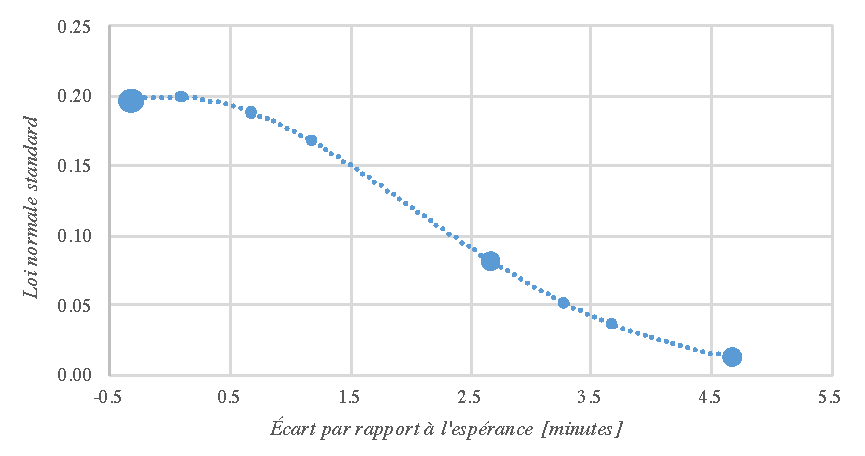
\includegraphics[width=\textwidth]{loiNormA.pdf}}
	\caption{Répartition des résultats de la première expérience (partie A) selon la loi normale centrée. L'aire des bulle est proportionnelle au nombre de résultats identiques.}
\end{figure}

\begin{figure}[h!] \centering{
		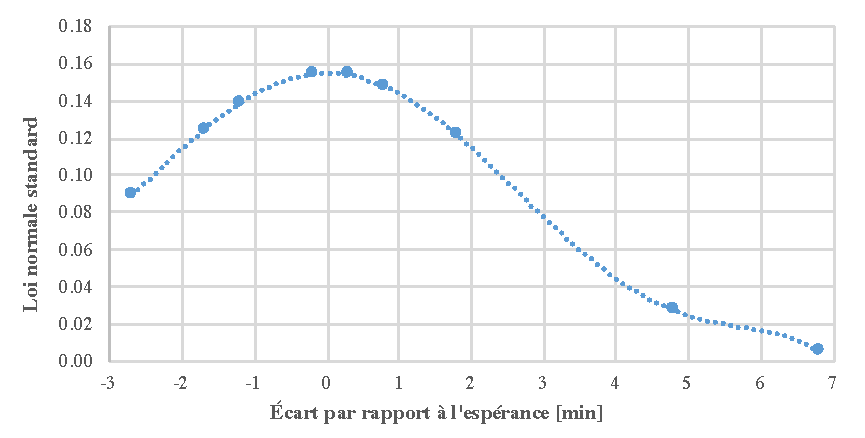
\includegraphics[width=\textwidth]{loiNormB.pdf}}
	\caption{Répartition des résultats de la première expérience (partie B) Bselon la loi normale centrée. L'aire des bulle est proportionnelle au nombre de résultats identiques.}
\end{figure}
\clearpage

\subsection{Expérience complémentaire} \label{ssec:exp2.2}
Cette expérience a pour but de tester l'intérêt suscité par les vidéos le rôle de variable dans l'expérience précédente

\newpage
\section{Seconde expérience} \label{sec:exp2}
Jusqu'à ce point, je ne me suis penché que sur le facteur émotionnel pour influencer le temps perçu par les volontaires ayant participé à mon expérience, leur travail étant d'estimer une durée imposée. Cette expérience est, au contraire, élaborée dans le but d'être opposée à la première : au lieu d'avoir à définir une durée, il faut la produire et la variable étudiée n'est pas de nature psychologique mais somatique.
% Jugement prospectif (avec horloge) =/= jugement rétrospectif 
\subsection{Expérience préparatoire} \label{ssec:but2.1}
Il est demandé à cet effet à des volontaires de se relaxer puis de faire de la corde à sauter. Après chacune de ces activités, ils doivent compter une durée qu'ils pensent être égale à celle demandée, l'objectif étant de déterminer si une activité physique modifie momentanément la perception temporelle par la comparaison des deux durées. Cette première partie de l'expérience, a pour but de tester le protocole défini ci-dessous et de l'adapter en fonction des résultats obtenus.

\subsection{Définition du protocole} \label{ssec:defProto2.1}

\subsubsection{Préparation} \label{sssec:preparation2.1}
Cette expérience ne requière que peu de matériel pour sa réalisation.

\begin{description}
	\item[Une trentaine de participants] L'expérience se déroule par petit groupes, selon la place disponible.
	\item[Une salle] Elle doit être pourvue d'un espace libre pour y effectuer une activité physique et ne doit fournir aucune indication temporelle; les horloges sont démontées, l'ordinateur de la classe et le projecteur sont éteints. Elle doit être assez grande pour la diviser en deux zones : une partie où l'on attend puis où l'on fait du sport et une autre où le sens du temps est testé. Cela évite qu'une personne en train de compter ne fournisse une durée de référence aux autres participants et qu'elle ne soit elle même perturbée par leur activité. 
	\item[Des cordes à sauter] Elles sont le moyen le plus simple faire effectuer des exercices aux volontaires, c'est un outil qui permet de produire un effort cardiovasculaire de façon efficace losque l'on dispose de peu d'espace pour faire du sport.
	\item[Un ordinateur] Dans le but d'atteindre la meilleure précision, les participants sont chargés de chronométrer eux-même le temps qu'il leur est demandé de produire. Il est par conséquent indispensable que l'outil utilisé n'affiche pas le temps compté. Une solution à ce problème est de placer un bout de scotch sur l'écran d'un chronomètre et de l'enlever lorsque l'on souhaite reporter le résultat dans un tableau. Cette astuce n'est cependant pas pratique car il faut à chaque fois replacer le masque, le scotch laisse des résidus de colle sur l'instrument et les relevés manuels des performances induisent un risque d'erreur lors de la copie. Pour éviter ces désagréments et être plus efficace lors de l'expérience, j'ai jugé utile d'utiliser une application pour chronométrer les participants. J'ai ainsi profité d'un forum sur lequel il est possible de demander à des developpeurs de programmer des logiciels selon des besoins spécifiques. Compte tenu de mon manque total de connaissance en programmation, un bienfaiteur anonyme répondant au nom de NoG5\footnote{\url{https://www.reddit.com/user/NoG5} sur le forum dédié aux requête relatives à la programmation \url{https://www.reddit.com/r/programmingrequests/}} m'a offert un outil très efficace en implémentant l'interface que je lui ai proposée. Ce logiciel permet d'enregistrer les résultats ainsi que les noms des participants dans un format qu'il est aisé de porter dans un tableur (voir page \pageref{sec:chrono}).
\end{description}

\subsubsection{Méthode} \label{sssec:methode2.1}
\begin{enumerate}
	\item Ménager un espace libre dans la salle en poussant certaines tables dans un coin.
	\item Installer l'ordinateur à l'opposé de cet espace et ouvrir le chronomètre.
	\item Rechercher un premier groupe de personne environ égal au nombre de cordes à sauter dont on dispose.
	\item Leur demander de s'asseoir jusqu'a ce qu'ils se sentent relaxés.
	\item Demander aux participants d'aller tour à tour s'asseoir devant l'ordinateur, d'entrer leur nom suivi de la mention «\,relaxé\,» et de compter pendant 10 secondes en appuyant sur le bouton \emph{Start} lorsqu'ils commencent puis sur \emph{Stop} lorsqu'ils ont fini.
	\item Distribuer une corde à sauter à chaque personne ayant terminé le premier test et leur demander de sauter de manière à produire un effort important.
	\item Quand le premier participant à avoir reçu sa corde commence à se fatiguer, lui demander de répéter l'expérience en mentionnant «\,échauffé\,» après son nom. Les autres suivent dans le même ordre qu'auparavant.
	\item Ouvrir le fichier contenant les résultats et les insérer dans un tableur.
	\item Recommencer l'expérience avec un nouveau groupe.
\end{enumerate}
% je préfères qu'ils se sentent eux même relaxés plutôt que je leur impose une durée de détente

\subsection{Résultats} \label{ssec:resultats2.1}

\begin{table}[h]
	\centering
	\caption{Résultats de l'expérience préparatoire} \label{tbl:exp2.1P}
	\begin{tabular}{llll}
		\toprule 
		\textbf{Nom} & \textbf{Temps 1 [s]} & \textbf{Temps 2 [s]} & \textbf{$\Delta$ temps [s]} \\ \midrule
		Ahmed & 8,62 & 9,39 & 0,77 \\
		Aliénor & 10,45 & 10,86 & 0,42 \\
		Barbara & 9,59 & 10,40 & 0,81 \\
		Imad & 8,80 & 9,86 & 1,06 \\
		Laura & 11,86 & 13,02 & 1,16 \\
		Sajinth & 12,48 & 13,41 & 0,93 \\
		Sarra & 11,05 & 12,70 & 1,65 \\ \bottomrule
	\end{tabular}
\end{table}

\subsection{Analyse} \label{ssec:analyse2.1}

\begin{table}[h]
	\centering
	\caption{Analyse des résultats de l'expérience préparatoire} \label{tbl:analyse2.1P}
	\begin{tabular}{ll}
		\toprule 
		\textbf{En fonction de la différence de temps} & \textbf{secondes [s]} \\ \midrule
		différence médiane & 0,93 \\
		différence moy & 0,97 \\
		valeur maximale & 1,65 \\
		valeur minimale & 0,42 \\ \bottomrule
	\end{tabular}
\end{table}

\subsubsection{Analyse critique} \label{sssec:analyseCrit2.1}
Cette expérience à petite échelle a été réalisée dans le but de mettre à l'épreuve le protocole précédemment défini, j'ai ainsi observé différents paramètres qui nécessitent d'être modifiés pour conduire au mieux l'expérience réelle. 

En premier lieu, il faut prendre garde au nombre de personnes qui participent en même temps à l'expérience. Il est très important ne faire participer que de petits groupes pour éviter qu'ils ne fassent la queue trop longtemps avant de pouvoir chronométrer leur premier temps, la suite de l'expérience n'en est d'ailleurs que facilitée car les sujets ont plus de place pour s'échauffer avec leur corde à sauter. Ils profitent aussi de ce faible effectif au moment de chronométrer leur temps pour la deuxième fois puisqu'ils ne doivent pas attendre.

\subsubsection{Analyse des résultats} \label{sssec:analyseResult2.1}
% CHERCHER COMBIEN DE TEMPS IL FAUT POUR SE REPOSER D'UN EFFORT PHYSIQUE !!!!
% effet psychologique => 2 mesures

\subsection{Expérience 2} \label{ssec:but2.2}

\subsection{Définition du protocole} \label{ssec:defProto2.1}

\subsubsection{Préparation} \label{sssec:preparation2.2}
\begin{description}
	\item[Une trentaine de participants]
\end{description}

\subsubsection{Méthode} \label{sssec:methode2.2}

\subsection{Résultats} \label{ssec:resultats2.2}

\begin{table}[h]
	\centering
	\caption{Résultats de l'expérience 2} \label{tbl:exp2.1}
	\begin{tabular}{llllll}
		\toprule
		\textbf{Nom} &  \multicolumn{2}{l}{\textbf{Temps moyen 1 [s]}}  & \multicolumn{2}{l}{\textbf{Temps moyen 2 [s]}} & \textbf{$\Delta$ temps moyen} \\ \midrule
		Aurélien & 9,69 & (10,11 \& 9,27) & 11,33 & (11,78 \& 10,88) & 1,64 \\
		Célia & 10,42 & (10,79 \& 10,06) & 10,65 & (10,08 \& 11,22) & 0,23 \\
		Damien & 7,69 & (7,28 \& 8,10) & 8,69 & (9,13 \& 8,24) & 1,00 \\
		Léana & 9,50 & (9,41 \& 9,59) & 8,90 & (9,34 \& 8,45) & -0,61 \\
		Louis & 10,91 & (9,17 \& 12,66) & 17,36 & (18,93 \& 15,79) & 6,44 \\
		Nils & 10,54 & (11,03 \& 10,05) & 10,28 & (10,35 \& 10,21) & -0,26 \\ \bottomrule
	\end{tabular}
\end{table}

\subsection{Analyse} \label{ssec:analyse2.2}

\subsubsection{Analyse critique} \label{sssec:analyseCrit2.2}

\subsubsection{Analyse des résultats} \label{sssec:analyseResult2.2}

\begin{table}[h!]
	\centering
	\caption{Analyse des résultats de l'expérience 2 (avec Louis)} \label{tbl:analyse2.1}
	\begin{tabular}{lll}
		\toprule 
		\textbf{En fonction de $\Delta$ temps moyen} & \textbf{Avec Louis [s]} & \textbf{Sans Louis [s]} \\ \midrule
		différence médiane & 0,61 & 0,23 \\
		différence moyenne & 1,41 & 0,40 \\
		valeur maximale & 6,44 & 1,64 \\
		valeur minimale & -0,61 & -0,61 \\ \bottomrule
	\end{tabular}
\end{table}

\newpage
\section{Réponse à la problématique} \label{sec:reponseProb}

\newpage
\section{Conclusion} \label{sec:conclusion}
% dire que je voulais faire plus d'expériences parler du top down bottom up
% conclusion du travail

% remerciements

%----------------------------------------------------------------------------------------
%	Annexes
%----------------------------------------------------------------------------------------

\chapterimage{head2.jpg}

\appendix
\chapter{Annexes} \label{cha:annexes}
\section*{Expérience 1}
\addcontentsline{toc}{section}{Expérience 1}

\subsection*{Sudoku} \label{sec:Sudoku}
\addcontentsline{toc}{subsection}{Sudoku}
\begin{figure}[htp] \centering{
		\includegraphics[trim=40 360 40 75, clip, width=\textwidth]{exp/Sudoku}} % gauche bas droite haut
	\caption{Sudoku distribué lors de l'expérience 1}
\end{figure}  

\newpage
\subsection*{Questionnaires} \label{sec:Questionnaires}
\addcontentsline{toc}{subsection}{Questionnaires}
\begin{figure}[htp] \centering{
		\includegraphics[trim=40 310 40 0,clip, width=\textwidth]{exp/QuestA}}
	\caption{Questionnaire distribué lors de la première partie de l'expérience 1}
\end{figure}

\newpage
\begin{figure}[htp] \centering{
		\includegraphics[trim= 40 310 40 0,clip, width=\textwidth]{exp/QuestB}}
	\caption{Questionnaire distribué lors de la seconde partie de l'expérience 1}
\end{figure}

\newpage
\section*{Expérience 2}
\addcontentsline{toc}{section}{Expérience 2}

\subsection*{Chronomètre} \label{sec:chrono}
\addcontentsline{toc}{subsection}{Sudoku}
\begin{figure}[htp] \centering{
		\includegraphics[width=\textwidth]{exp/mockup}}
	\caption{Interface du chronomètre utilisé lors de l'expérience 2}
\end{figure}
Le logiciel en question est disponible aux adresses suivantes :
\begin{itemize}
\item \url{http://nog5.com/files/request20.v2.exe} (serveur de l'auteur)
\item \url{https://github.com/Temporalite/TM/tree/master/exp%C3%A9rience/2/Timer.exe} (page GitHub du projet)
\end{itemize}

%----------------------------------------------------------------------------------------
%	Bibliographie
%----------------------------------------------------------------------------------------

\chapterimage{head1.jpg} % Chapter heading image

\chapter{Bibliographie}
Références non présentes dans le texte mais qu'il faudra bien placer un jour : \cite{ref1} \cite{vidnul} \cite{vidcool} \cite{imgtitre} \cite{imgheader1} \cite{analysedonnees}

\begin{remark}
	Les images et autres ressources issues d'internet utilisées dans ce travail ne sont, sauf indication contraire, pas restreintes d'usage pour une utilisation non commerciale.
\end{remark}

\section*{Livres}
\addcontentsline{toc}{section}{Livres}
\printbibliography[heading=bibempty,type=book]
\section*{Articles}
\addcontentsline{toc}{section}{Articles}
\printbibliography[heading=bibempty,type=article]
\section*{Non publié}
\addcontentsline{toc}{section}{Non publié}
\printbibliography[heading=bibempty,type=unpublished]
\section*{Ressources en ligne}
\addcontentsline{toc}{section}{Ressources en ligne}
\printbibliography[heading=bibempty,type=online]

%----------------------------------------------------------------------------------------


%EXEMPLE DE NOTEs DE BAS DE PAGE QUI PRENNENT TROP DE PLACE
% \footnote[200]{John. H. WEARDEN et Bairbre MCSHANE. «\,Interval production as an analogue of the peak procedure : Evidence for similarity of human and animal timing processes\,». In : The Quarterly Journal of Experimental Psychology Section B 40.4 (oct. 1988), pages 363–375}
% \footnote[201]{ibid}
% \footnote[202]{ibid}
% \footnote[203]{Catalin V. BUHUSI et Warren H. MECK. «\,What makes us tick ? Functional and neural mechanisms of interval timing\,». In : Nature Reviews Neuroscience 6.10 (oct. 2005), pages 755-765}
% \footnote[204]{op cit John. H. WEARDEN (1998)}
% \footnote[205]{ibid}
% \footnote[206]{Sylvie DROIT-VOLET. «\,Time perception, emotions and mood disorders\,». In : Journal of Physiology-Paris 107.4 (sept. 2013), pages 255-264}


\end{document}
